\chapter{Introduction to the constructive gravity programme}

\section{The r\^ole of gravity in physics}
As the title suggests, this thesis is primarily concerned with \emph{gravity}. In the ensemble of physical theories, gravity plays a special r\^ole. It serves a different purpose than the theories we will call \emph{matter theories}. The latter are subject to direct observations: photons---quanta of the electomagnetic field---hit the observers retina, allowing her to make inferences about the source of the particles. Charged fermions---again quanta of a corresponding matter field---induce signals in a semiconductor detector. Specific signatures in the signals may be associated with certain events that contributed to the production of the incident fermions, such that the statistics of these observations is able to falsify hypotheses about the underlying mechanisms.

How does gravity fit into this picture? The revolution of a binary star about its center of mass, commonly known to be caused by gravity, is not observed directly. Neither are its gravitational spin-up and eventual merger. Rather, the stars emit photons that are picked up by the astronomer, who concludes details about the trajectories. When the LIGO and Virgo Collaborations announced the first observation of gravitational waves \cite{ligo}, the ground-breaking detection was earth-bound, but in a certain sense not \emph{direct}: it amounts to the analysis of interference patterns from photons that bounced off of mirrors at the end of the detector arms. General relativity predicts that these arms should expand and contract under the influence of incident gravitational waves. Eventually, the signature in the interference pattern was found to match the predictions for a binary black hole merger.

\begin{figure}
  \begin{center}
    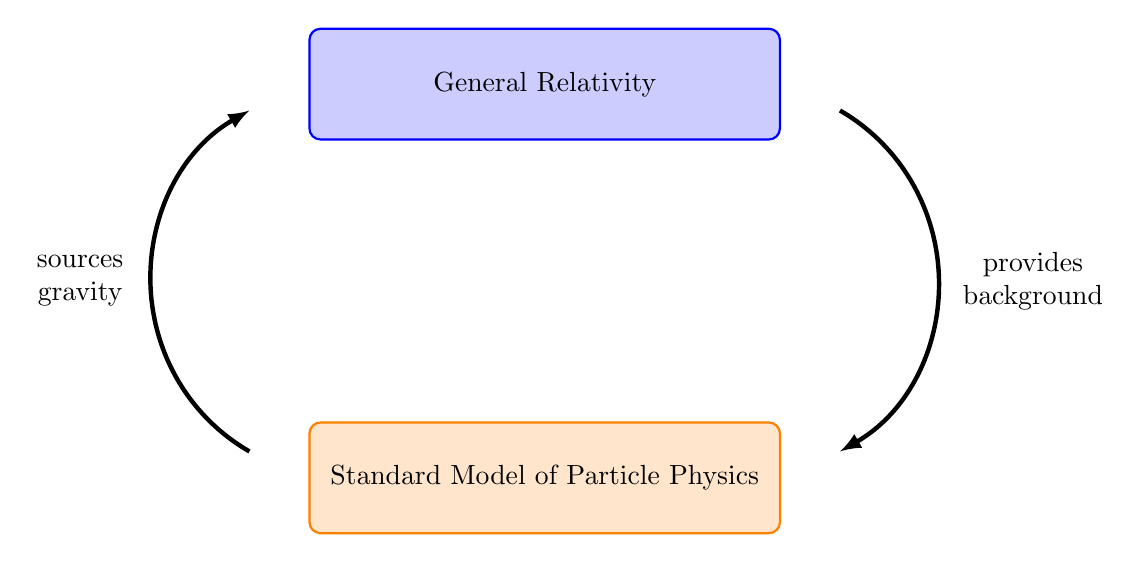
\begin{tikzpicture}[%
      auto,
      block1/.style={rectangle,thick,draw=blue,fill=blue!20,align=center,rounded corners,minimum width=17em,minimum height=4em},
      block2/.style={rectangle,thick,draw=orange,fill=orange!20,align=center,rounded corners,minimum width=17em,minimum height=4em},
      pics/carc/.style args={#1:#2:#3}{code={\draw[pic actions] (#1:#3) arc(#1:#2:#3);}}
      ]
      \draw (0,2.5) node[block1] (G) {General Relativity};
      \draw (0,-2.5) node[block2] (S) {Standard Model of Particle Physics};
      \draw (-2.5,0) pic[latex-,ultra thick]{carc=120:240:2.5};
      \draw (2.5,0) pic[latex-,ultra thick]{carc=-60:60:2.5};
      \draw (-5.9,0) node[align=center] {sources\\gravity};
      \draw (6.2,0) node[align=center] {provides\\background};
    \end{tikzpicture}
  \end{center}
  \label{figure_smpp_gr}
  \caption{Interplay of the standard model theories and general relativity. Matter content sources the gravitational field equations. The gravitational field, in turn, provides the background on which matter fields propagate. Together, this yields a highly accurate fundamental description of the universe.}
\end{figure}

From this point of view, gravity sets the stage for the propagation of matter fields. This is witnessed by the dynamics for matter fields, one example of which is the electromagnetic potential in Maxwell electrodynamics. Its field equations are derived from the action functional
\begin{equation*}
  S_\text{Maxwell}\lbrack A\rbrack = \int\mathrm d^4x \sqrt{-g} g^{ac} g^{bc} F_{ab} F_{cd},
\end{equation*}
which depends on the potential $A$ via the field strength tensor $F = \mathrm dA$. Maxwell's theory of the electromagnetic field has been a huge success as it is the foundation of many applications throughout science. The quantum field theories for the electromagnetic field and similar gauge theories, together with the fermonic sector, form the standard model of particle physics (SMPP), which is widely regarded as the most precisely tested physical theory\footnote{For example, the magnetic moment of the electron has been measured as $g/2 = 1.001\,159\,652\,180\,73(28)$. \cite{http://dx.doi.org/10.1103/PhysRevA.83.052122} Its value as proposed by quantum electrodynamics has been calculated as $g/2 = 1.001\,159\,652\,182\,03(73)$ \cite{https://doi.org/10.1103/PhysRevD.96.019901}. Both the experimentally measured value and the value calculated from quantum electrodynamics agree to more than 12 significant figures.}. Still, these matter theories presuppose knowledge of the spacetime metric $g$ which enters the action for the electromagnetic field above and contributes to other theories of the SMPP in a similar way. Consequently, the SMPP alone lacks \emph{predictivity}: collecting initial data of all physical fields is not enough for the physicist in order to determine the fields in the future, since the metric tensor has to be specified externally. 

One of the many great contributions by Einstein was the prescription of field equations that govern the dynamics of the metric tensor. \cite{einstein_gr} This theory is called \emph{general relativity} and may be derived from the Einstein-Hilbert action functional
\begin{equation*}
  S_\text{Einstein-Hilbert}\lbrack g\rbrack = \int\mathrm \mathrm d^4x \sqrt{-g} R.
\end{equation*}
Einstein's theory provides the missing link between matter and gravity, completing the SMPP to the joint model of SMPP and general relativity sketched in Fig.~\ref{figure_smpp_gr}, which is now predictive. It has also been verified numerous times, both via astronomical observations and \emph{in terra}\footnote{earthbound} experiments, albeit to a lesser degree of certainty\footnote{Only four significant figures of the gravitational constant are known. \cite{https://doi.org/10.1103/FRevModPhys.88.035009} Measurements with higher precision yield conflicting results. \cite{https://doi.org/10.1103/RevModPhys.84.1527}}.

Of course, the division of physical theories into matter theories and gravity is only a \emph{metaphysical} notion. Both make testable predictions about the outcome of experiments; both have been shown to accurately describe reality in a variety of circumstances. But exactly in this metaphysical idea lies the mindset of \emph{constructive gravity}, which seeks to address the search for other (more?) complete pictures of matter and gravity.

\section{Modified gravity from refined matter theories}
Under certain assumptions, Einstein's general relativity is the unique theory that completes the SMPP to a predictive theory of matter and gravity.\cite{lovelock,hkt,deser} Only two unknown parameters need to be fixed: Newton's gravitational constant and the cosmological constant.

\begin{itemize}
\item motto: matter tells gravity how to curve, gravity tells matter how to move -> lift to theory level
\item 2d plot of theories?
\item what could hint at the existence of refined matter theories?
\item dark matter
\end{itemize}

\section{Canonical and covariant approaches to constructive gravity}

\begin{itemize}
\item canonical approach: implementing the constraint algebra
\item a success story, but does it keep its promises?
\item covariant view: equivalent and complementary
\item simpler?
\end{itemize}

Two kinds of inconsistencies: Within the SMs -> quantum gravity inevitable? But also pheno that does not match SM -> closure?

We only ever so slightly deviate from the established models about matter and gravity. For example, where the standard model is restricted to field equations of second derivative, we keep this restriction. This is not because other efforts are not deemed worthwile---they certainly are, but should be explored \emph{ceteris paribus}, one at a time. Our focus lies on novel matter theories and their gravitational implications \emph{within the existing meta-theory of classical physics}.

\textbf{game plan: structure of the thesis}
